% Title: glps_renderer figure
% Creator: GL2PS 1.3.8, (C) 1999-2012 C. Geuzaine
% For: Octave
% CreationDate: Wed Mar 23 19:36:50 2016
\setlength{\unitlength}{0.42pt}
\begin{picture}(0,0)
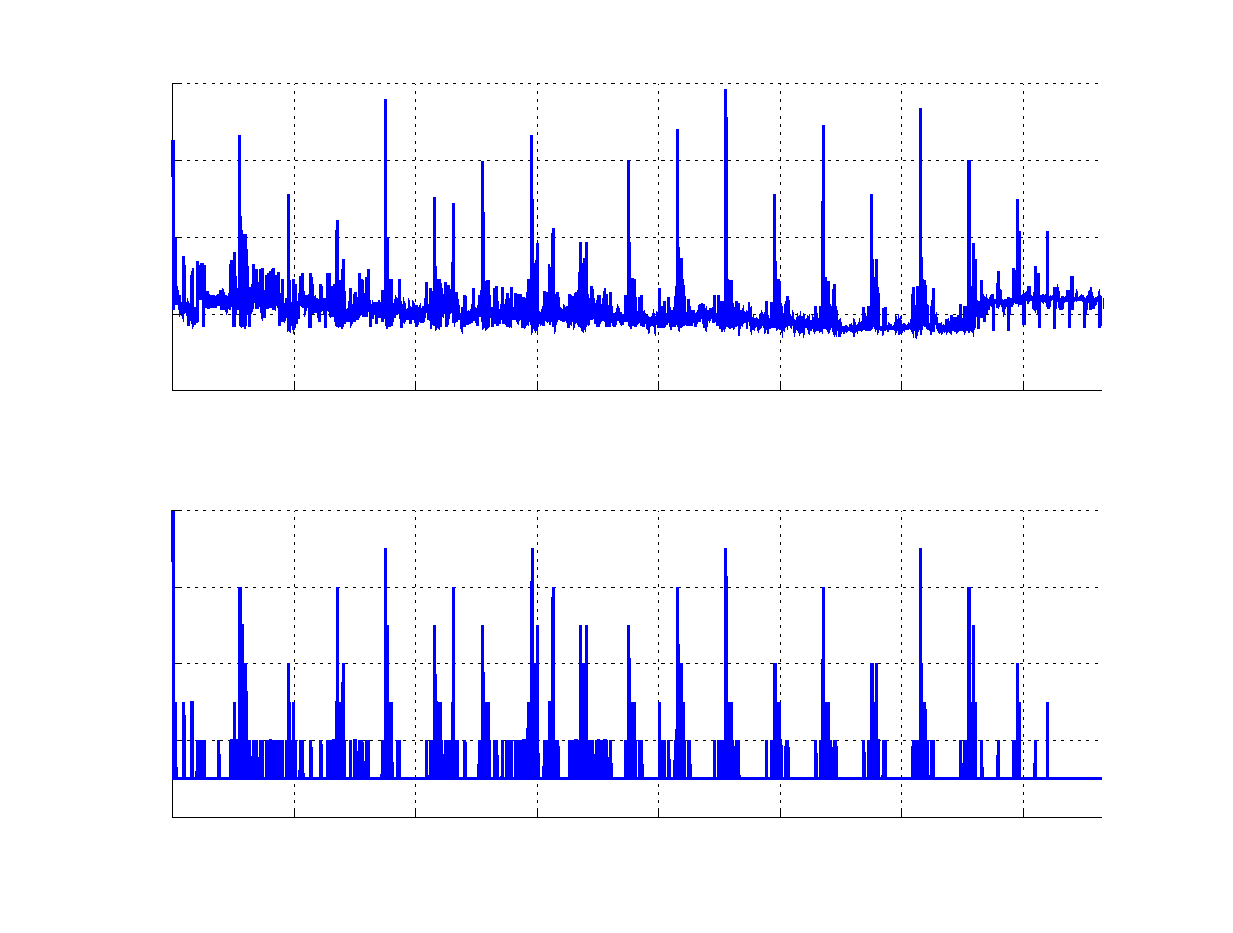
\includegraphics[trim=30  20   0   0,clip,scale=0.42]{time_16_02_03_N16_nodist-inc}
\end{picture}%
\begin{picture}(546, 412)(30,20)
\fontsize{8}{0}
\selectfont\put(74.88,247.205){\makebox(0,0)[t]{\textcolor[rgb]{0,0,0}{{0}}}}
\fontsize{8}{0}
\selectfont\put(133.214,247.205){\makebox(0,0)[t]{\textcolor[rgb]{0,0,0}{{2}}}}
\fontsize{8}{0}
\selectfont\put(191.548,247.205){\makebox(0,0)[t]{\textcolor[rgb]{0,0,0}{{4}}}}
\fontsize{8}{0}
\selectfont\put(249.882,247.205){\makebox(0,0)[t]{\textcolor[rgb]{0,0,0}{{6}}}}
\fontsize{8}{0}
\selectfont\put(308.216,247.205){\makebox(0,0)[t]{\textcolor[rgb]{0,0,0}{{8}}}}
\fontsize{8}{0}
\selectfont\put(366.549,247.205){\makebox(0,0)[t]{\textcolor[rgb]{0,0,0}{{10}}}}
\fontsize{8}{0}
\selectfont\put(424.883,247.205){\makebox(0,0)[t]{\textcolor[rgb]{0,0,0}{{12}}}}
\fontsize{8}{0}
\selectfont\put(483.217,247.205){\makebox(0,0)[t]{\textcolor[rgb]{0,0,0}{{14}}}}
\fontsize{8}{0}
\selectfont\put(69.8755,252.218){\makebox(0,0)[r]{\textcolor[rgb]{0,0,0}{{0}}}}
\fontsize{8}{0}
\selectfont\put(69.8755,289.063){\makebox(0,0)[r]{\textcolor[rgb]{0,0,0}{{1}}}}
\fontsize{8}{0}
\selectfont\put(69.8755,325.909){\makebox(0,0)[r]{\textcolor[rgb]{0,0,0}{{2}}}}
\fontsize{8}{0}
\selectfont\put(69.8755,362.754){\makebox(0,0)[r]{\textcolor[rgb]{0,0,0}{{3}}}}
\fontsize{8}{0}
\selectfont\put(69.8755,399.6){\makebox(0,0)[r]{\textcolor[rgb]{0,0,0}{{4}}}}
\fontsize{8}{0}
\selectfont\put(48.8755,325.909){\rotatebox{90}{\makebox(0,0)[b]{\textcolor[rgb]{0,0,0}{{comp. time $[ms]$}}}}}
\fontsize{8}{0}
\selectfont\put(74.88,42.507){\makebox(0,0)[t]{\textcolor[rgb]{0,0,0}{{0}}}}
\fontsize{8}{0}
\selectfont\put(133.214,42.507){\makebox(0,0)[t]{\textcolor[rgb]{0,0,0}{{2}}}}
\fontsize{8}{0}
\selectfont\put(191.548,42.507){\makebox(0,0)[t]{\textcolor[rgb]{0,0,0}{{4}}}}
\fontsize{8}{0}
\selectfont\put(249.882,42.507){\makebox(0,0)[t]{\textcolor[rgb]{0,0,0}{{6}}}}
\fontsize{8}{0}
\selectfont\put(308.216,42.507){\makebox(0,0)[t]{\textcolor[rgb]{0,0,0}{{8}}}}
\fontsize{8}{0}
\selectfont\put(366.549,42.507){\makebox(0,0)[t]{\textcolor[rgb]{0,0,0}{{10}}}}
\fontsize{8}{0}
\selectfont\put(424.883,42.507){\makebox(0,0)[t]{\textcolor[rgb]{0,0,0}{{12}}}}
\fontsize{8}{0}
\selectfont\put(483.217,42.507){\makebox(0,0)[t]{\textcolor[rgb]{0,0,0}{{14}}}}
\fontsize{8}{0}
\selectfont\put(69.8755,47.52){\makebox(0,0)[r]{\textcolor[rgb]{0,0,0}{{0}}}}
\fontsize{8}{0}
\selectfont\put(69.8755,84.3656){\makebox(0,0)[r]{\textcolor[rgb]{0,0,0}{{2}}}}
\fontsize{8}{0}
\selectfont\put(69.8755,121.211){\makebox(0,0)[r]{\textcolor[rgb]{0,0,0}{{4}}}}
\fontsize{8}{0}
\selectfont\put(69.8755,158.057){\makebox(0,0)[r]{\textcolor[rgb]{0,0,0}{{6}}}}
\fontsize{8}{0}
\selectfont\put(69.8755,194.902){\makebox(0,0)[r]{\textcolor[rgb]{0,0,0}{{8}}}}
\fontsize{8}{0}
\selectfont\put(298.08,9.50697){\makebox(0,0)[t]{\textcolor[rgb]{0,0,0}{{simulation time $[s]$}}}}
\fontsize{8}{0}
\selectfont\put(48.8755,121.211){\rotatebox{90}{\makebox(0,0)[b]{\textcolor[rgb]{0,0,0}{{num. of iterations}}}}}
\end{picture}
